\documentclass{beamer}

\title{Model Antrian \textit{Multi-Server:} M/M/c}
\subtitle{dengan Pengantar Model Stokastik dan Teori Antrian \\ dengan R dan QtsPlus \\ (Revisi)}
\author{Bisma Rohpanca Joyosumarto (2106635581)}
\institute{Departemen Matematika FMIPA UI \\ Universitas Indonesia}
\date{
    November 2024

    Riset Operasi
    
    Tahun Ajaran 2024/2025 Semester Ganjil
}

% === bismastyle.sty ===
%\usetheme{Copenhagen}

\AtBeginSection[]
{
  \begin{frame}{Daftar isi keseluruhan}
    \tableofcontents[currentsection]
  \end{frame}
}

\AtBeginSubsection[]{
  \frame<beamer>{ 
    \frametitle{Daftar isi di bab}   

\tableofcontents[currentsection,currentsubsection,sectionstyle=show/hide,subsectionstyle=show/shaded/hide,subsubsectionstyle=show/show/shaded/shaded]}
}
% sumber: https://tex.stackexchange.com/questions/434088/beamer-toc-on-each-subsection

\addtobeamertemplate{navigation symbols}{}{%
    \usebeamerfont{footline}%
    \usebeamercolor[fg]{footline}%
    \hspace{1em}%
    \insertframenumber/\inserttotalframenumber
}

\newcommand{\pars}[1]{\left(#1\right)}
\newcommand{\brackets}[1]{\left[#1\right]}
\newcommand{\braces}[1]{\left\{#1\right\}}

\usepackage{hyperref}
\usepackage{graphicx}
\usepackage{amsmath}

\usepackage{minted}
% === akhir bismastyle.sty ===

\begin{document}

\frame{\titlepage}

\begin{frame}{Daftar isi keseluruhan}
    \tableofcontents
\end{frame}

\section[Pengantar Model Stokastik dan Teori Antrian. dengan praktik di R]{Pengantar Model Stokastik dan Teori Antrian \\ dengan praktik di R}

\begin{frame}{\textit{Overview:} Teori Antrian dan Model Stokastik}
    \begin{itemize}
        \item Dalam suatu \textbf{antrian \textit{(queue)}}, orang bisa masuk mengantri, dilayani, kemudian meninggalkan antrian
        \item Apabila ada beberapa pelayan, tiap baris/pelayan disebut \textit{server}, sehingga secara keseluruhan, terdapat satu antrian dengan sejumlah \textit{server}
        \item Pada dasarnya, proses mengantri bisa dimodel dengan melihat dua aspek: proses datangnya orang, dan proses perginya orang
        \item Di kuliah Pengantar Sains Data (Metode Statistika), kita sudah kenal \textbf{distribusi Poisson} yang memodelkan probabilitas banyaknya kemunculan dalam suatu satuan waktu, dalam yang namanya \textbf{proses Poisson}
        \item Baik datangnya orang maupun perginya orang, masing-masing bisa dimodelkan sebagai proses Poisson: datangnya orang sama saja kemunculan di pintu masuk, dan perginya orang sama saja kemunculan di pintu keluar
    \end{itemize}
\end{frame}

\begin{frame}{\textit{Overview:} Proses Poisson dan Rantai Markov}
    \begin{itemize}
        \item Sifat utama proses Poisson adalah \textbf{sifat Markov} atau \textbf{sifat \textit{memoryless:}} probabilitas kedatangan \textbf{hanya bergantung pada kondisi saat itu}, tidak pada kondisi di masa lalu
        \item Proses Poisson adalah contoh \textbf{rantai Markov waktu kontinu} atau \textbf{\textit{continuous-time Markov chain} (CTMC)}
        \item CTMC itu sendiri adalah perumuman dari \textbf{rantai Markov waktu diskrit} atau \textbf{\textit{discrete-time Markov chain} (DTMC)}
        \item Agar lebih paham dasar statistik untuk teori antrian, termasuk mengapa distribusi Poisson dan distribusi eksponensial sering digunakan, mari kita bahas dari awal!
    \end{itemize}
\end{frame}

\subsection{Rantai Markov Waktu Diskrit (DTMC)}

\begin{frame}{Definisi DTMC}
    Secara umum, dalam suatu rantai Markov, ada sejumlah kemungkinan "keadaan" \textit{(state)}, ada waktu, dan ada probabilitas berpindah dari suatu \textit{state} ke \textit{state} lain di tiap waktu berikutnya.

    Suatu DTMC, misal ditulis \( \braces{X_t} \), terdiri dari
    \begin{itemize}
        \item Suatu \textit{state space} atau himpunan \textit{state}, misal \( S \), 
        %berisi semua "keadaan" \textit{(state)} yang mungkin
        yang terhitung (bisa berhingga)
        \item Himpunan indeks waktu, biasanya \( T = \braces{0, 1, 2, \dots} \)
        \item $X_t$ sebagai variabel acak untuk tiap \( t \in T \), yang nilainya bisa berupa \textit{state} apapun dari \( S \). Sehingga, \( \braces{X_t} \) adalah barisan variabel acak
    \end{itemize}
    dan memenuhi \textbf{sifat Markov} \textbf{(\textit{Markov property})} atau \textbf{\textit{memoryless property}} sebagai berikut:
    \begin{align*}
        \text{Pr}&\braces{X_{n+1} = j \, \mid \, X_0 = i_0, \, \dots \, X_{n-1} = i_{n-1}, X_n = i} \\
        &= \text{Pr}\braces{X_{n+1} = j \, \mid \, X_n = i}
    \end{align*}
    Artinya: probabilitas nilai \( X_t \) di waktu ke-\(\pars{n+1}\) hanya bergantung pada probabilitas di waktu ke-\(n\). Seolah-olah, tidak ada ingatan sama sekali tentang apa yang terjadi sebelum waktu ke-\(n\).

    %DTMC adalah contoh \textbf{proses stokastik \textit{(stochastic process)}}.
\end{frame}

\begin{frame}{DTMC stasioner}
    \begin{itemize}
        \item Kita bisa notasikan
        \[ P_{ij}^{n,n+1} = \text{Pr}\braces{X_{n+1} = j \, \mid \, X_n = i} \]
        yang disebut \textit{one-step transition probability}, dari \(X_n\) yang berada di \textit{state} \(i\) menjadi \(X_{n+1}\) yang berada di \textit{state} \(j\)
        \item Apabila nilai \(P_{ij}\) \textbf{tidak tergantung kapan}, maka rantai Markov disebut \textbf{stasioner}, dengan \textit{stationary transition probabilities}
        \item Dengan demikian, kita bisa menyusun \textbf{\textit{transition probability matrix} (TPM)} sebagai berikut, misalkan \(S=\braces{0,1,2,\dots}\):
        \[ P = \begin{pmatrix}
            P_{00} & P_{01} & P_{02} & \dots \\
            P_{10} & P_{11} & P_{12} & \dots \\
            \vdots & \vdots & \vdots & \ddots
        \end{pmatrix} \]
        dengan
        \[ P_{ij} = \text{Pr}\braces{X_{n+1} = j \, \mid \, X_n = i} \]
        sehingga baris ke-\(i\), kolom ke-\(j\) mengandung probabilitas transisi dari \textit{state} \(i\) ke \textit{state} \(j\).
    \end{itemize}
\end{frame}

\begin{frame}{Contoh DTMC stasioner: \textit{A Shoeshine Shop}}
    Misalkan ada usaha kecil oles sepatu. Hanya ada satu pelayan dan dua kursi pelanggan.
    \begin{itemize}
        \item Apabila kedua kursi kosong, orang cenderung tidak sadar bahwa itu adalah tempat oles sepatu, sehingga tidak datang.
        \item Namun, ketika salah satu kursi terisi, probabilitas kursi lainnya ikut terisi menjadi dua kali lipat dari biasanya.
        \item Ketika ada dua pelanggan, probabilitas satu pelanggan selesai adalah empat kali probabilitas keduanya belum selesai.
        \item Misalkan juga, tidak mungkin dua pelanggan datang sekaligus ataupun selesai sekaligus, dan tidak mungkin selesainya satu orang langsung diikuti datangnya pelanggan baru.
    \end{itemize}

    Ada empat keadaan yang mungkin, misalnya \( S = \braces{0,1,2,3} \) sebagai berikut
    \begin{enumerate}
        \item[(0)] Kedua kursi kosong
        \item[(1)] Kursi pertama saja diisi
        \item[(2)] Kursi kedua saja diisi
        \item[(3)] Kedua kursi diisi
    \end{enumerate}
\end{frame}

\begin{frame}{TPM untuk Contoh DTMC}
    TPM dari situasi di atas adalah seperti berikut:
    \[ P = \begin{pmatrix}
        0.5 & 0.25 & 0.25 & 0 \\
        0.25 & 0.25 & 0 & 0.5 \\
        0.25 & 0 & 0.25 & 0.5 \\
        0 & 0.4 & 0.4 & 0.2
    \end{pmatrix} \]
    Perhatikan bahwa sumasi tiap baris adalah satu. Ini akibat sifat probabilitas. Dari suatu \textit{state} \(i\), dia bisa ke \textit{state} lainnya (atau bahkan tetap di \textit{state} yang sama) dengan probabilitas tiap kemungkinan ke \textit{state} \(j\) sesuai baris ke-\(i\).
\end{frame}

\begin{frame}{Diagram Transisi untuk Contoh DTMC}
    TPM bisa divisualisasikan sebagai \textbf{diagram transisi} atau \textbf{\textit{transition diagram}} sebagai berikut

    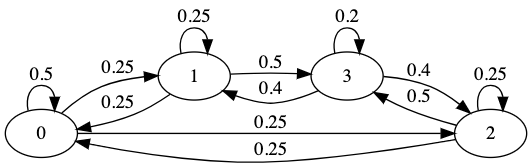
\includegraphics[scale=0.5]{gambar/contoh_dtmc.png}

    \begin{itemize}
        \item Tiap simpul melambangkan \textit{state}
        \item Tiap busur dari \(i\) ke \(j\) melambangkan transisi, dengan label \(P_{ij}\)
        \item Transisi dengan probabilitas nol tidak digambarkan
    \end{itemize}
    \textit{Fun fact:} rantai Markov adalah versi probabilistik dari automata hingga.
\end{frame}

\begin{frame}{Perbandingan: Diagram Transisi untuk Antrian}
    %Sedikit demi sedikit, kita coba lebih memahami teori antrian.
    Sebagai perbandingan dengan konsep antrian, perhatikan gambar berikut!

    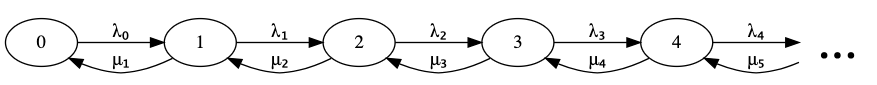
\includegraphics[scale=0.5]{gambar/diagram_transisi_antrian.png}

    Ini adalah diagram transisi yang umum dikenal untuk antrian.
    \begin{itemize}
        \item Himpunan \textit{state} \( S = \{ 0, 1, 2, 3, \dots \} \) menyatakan banyaknya orang (yang sedang mengantri) di antrian.
        \item Probabilitas \( P_{i,i+1} \), yaitu ketika banyaknya orang bertambah satu dari \( i \) (menjadi \( i+1 \) orang), ditulis \( \lambda_i \)
        \item Probabilitas \( P_{i,i-1} \), yaitu ketika banyaknya orang berkurang satu dari \( i \) (menjadi \( i-1 \) orang), ditulis \( \mu_i \)
    \end{itemize}
    Kita akan lihat nanti, notasi huruf \( \lambda \) tidak sembarangan dipilih.
\end{frame}

% Simulasi dan Analisis DTMC di R
\begin{frame}[fragile]{DTMC di R dengan \textit{package} markovchain}
    DTMC tergolong model stokastik (juga disebut proses stokastik) karena sifatnya yang probabilistik, sehingga menjadi pembahasan di ranah statistika (hingga menjadi kuliah Model Stokastik 1). Oleh karena itu, model stokastik seperti DTMC bisa disimulasikan di bahasa pemrograman R yang biasa digunakan oleh statistikawan. 
    
    Untuk DTMC, kita bisa gunakan \textit{package} markovchain:

\begin{minted}{r}
# install kalau belum
#install.packages("markovchain")

library("markovchain")
\end{minted}

    (Nanti akan ada \textit{package} khusus untuk simulasi antrian.)
\end{frame}

\begin{frame}[fragile]{Contoh DTMC di R}
    Kita bisa susun TPM dari contoh DTMC yang telah dibahas, sebagai berikut:

\begin{minted}{r}
mc1_P <- matrix(
  c(0.5,  0.25, 0.25, 0,
    0.25, 0.25, 0,    0.5,
    0.25, 0,    0.25, 0.5,
    0,    0.4,  0.4,  0.2),
  nrow = 4,
  byrow = TRUE
)
\end{minted}

Karena opsi \verb|byrow = TRUE|, matriks yang terbentuk akan seperti tertulis. Perhatikan bahwa dipasang \verb|nrow = 4| agar R tidak salah membaca data yang diberikan, yaitu agar matriks memiliki 4 (empat) baris.
\end{frame}

\begin{frame}[fragile]{Contoh DTMC di R}
    Setelah menyusun TPM, kita bisa mendefinisikan isi himpunan \(S\),

\begin{minted}{r}
mc1_states <- c("0", "1", "2", "3")
\end{minted}
    kemudian membuat objek \verb|markovchain| atau DTMC seperti berikut:

\begin{minted}{r}
mc1_obj <- new("markovchain",
               states = mc1_states,
               transitionMatrix = mc1_P)    
\end{minted}

    Informasi \textit{states} dan TPM bisa diperoleh kembali dengan mengetik nama objeknya:

\begin{minted}{r}
mc1_obj
\end{minted}

    Untuk memperoleh informasi \textit{states} saja, bisa digunakan fungsi \verb|states|

\begin{minted}{r}
states(mc1_obj)
\end{minted}

    Selain itu, diagram transisi juga bisa ditampilkan (lihat \textit{slide} berikutnya) dengan fungsi \verb|plot| seperti berikut.

\begin{minted}{r}
plot(mc1_obj)
\end{minted}
\end{frame}

\begin{frame}{Plot Diagram Transisi di R}
    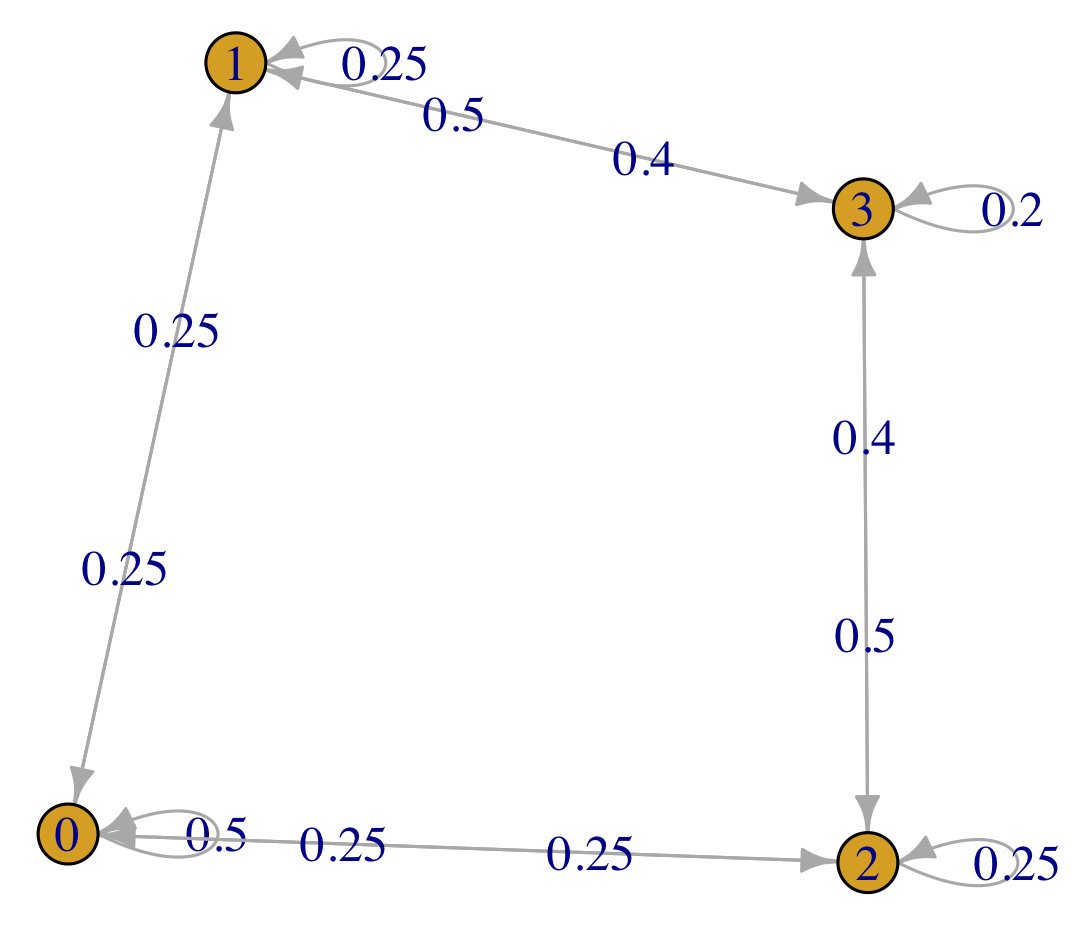
\includegraphics[scale=0.9]{gambar/contoh_dtmc_plot.png}
\end{frame}

\begin{frame}[fragile]{Simulasi DTMC di R}
    Untuk melakukan simulasi, tentukan waktu berjalannya simulasi,

\begin{minted}{r}
mc1_t <- 10    
\end{minted}

    kemudian lakukan \verb|set.seed| dengan bilangan bulat apapun, untuk keperluan \textit{reproducibility} (agar hasil selalu sama walaupun \textit{random}), misalnya 123:

\begin{minted}{r}
set.seed(123)
\end{minted}

    Barulah lakukan simulasi dengan fungsi \verb|rmarkovchain|, misalnya dengan \textit{state} awal "0"

\begin{minted}{r}
mc1_sim <- rmarkovchain(n = mc1_t, object = mc1_obj,
                        t0 = "0")
\end{minted}

Untuk \textit{random seed} yang dipilih yaitu 123, hasil simulasi yang tersimpan di \verb|mc1_sim| adalah 10 \textit{state} berikut, secara berturut-turut:

\verb|"0" "2" "3" "3" "3" "1" "0" "2" "0" "0"|

\end{frame}

\begin{frame}[fragile]{Plot Hasil Simulasi DTMC di R}
    Dengan sedikit kode, kita dapat membuat \textit{plot} hasil simulasi tersebut (ditampilkan di \textit{slide} selanjutnya).

\begin{minted}{r}
mc1_sim_factors <- factor(mc1_sim, levels = mc1_states)
mc1_sim_int <- as.integer(mc1_sim_factors)
mc1_sim_times <- 1 : mc1_t
plot(x = mc1_sim_times,
     y = mc1_sim_int,
     xlab = "Waktu (diskrit)",
     ylab = "State",
     main = "Simulasi DTMC",
     xaxt = "n", yaxt = "n")
axis(1, at = mc1_sim_times)
axis(2, at = 1 : length(mc1_states),
        labels = mc1_states)
\end{minted}
\end{frame}

\begin{frame}{Plot Hasil Simulasi DTMC di R}
    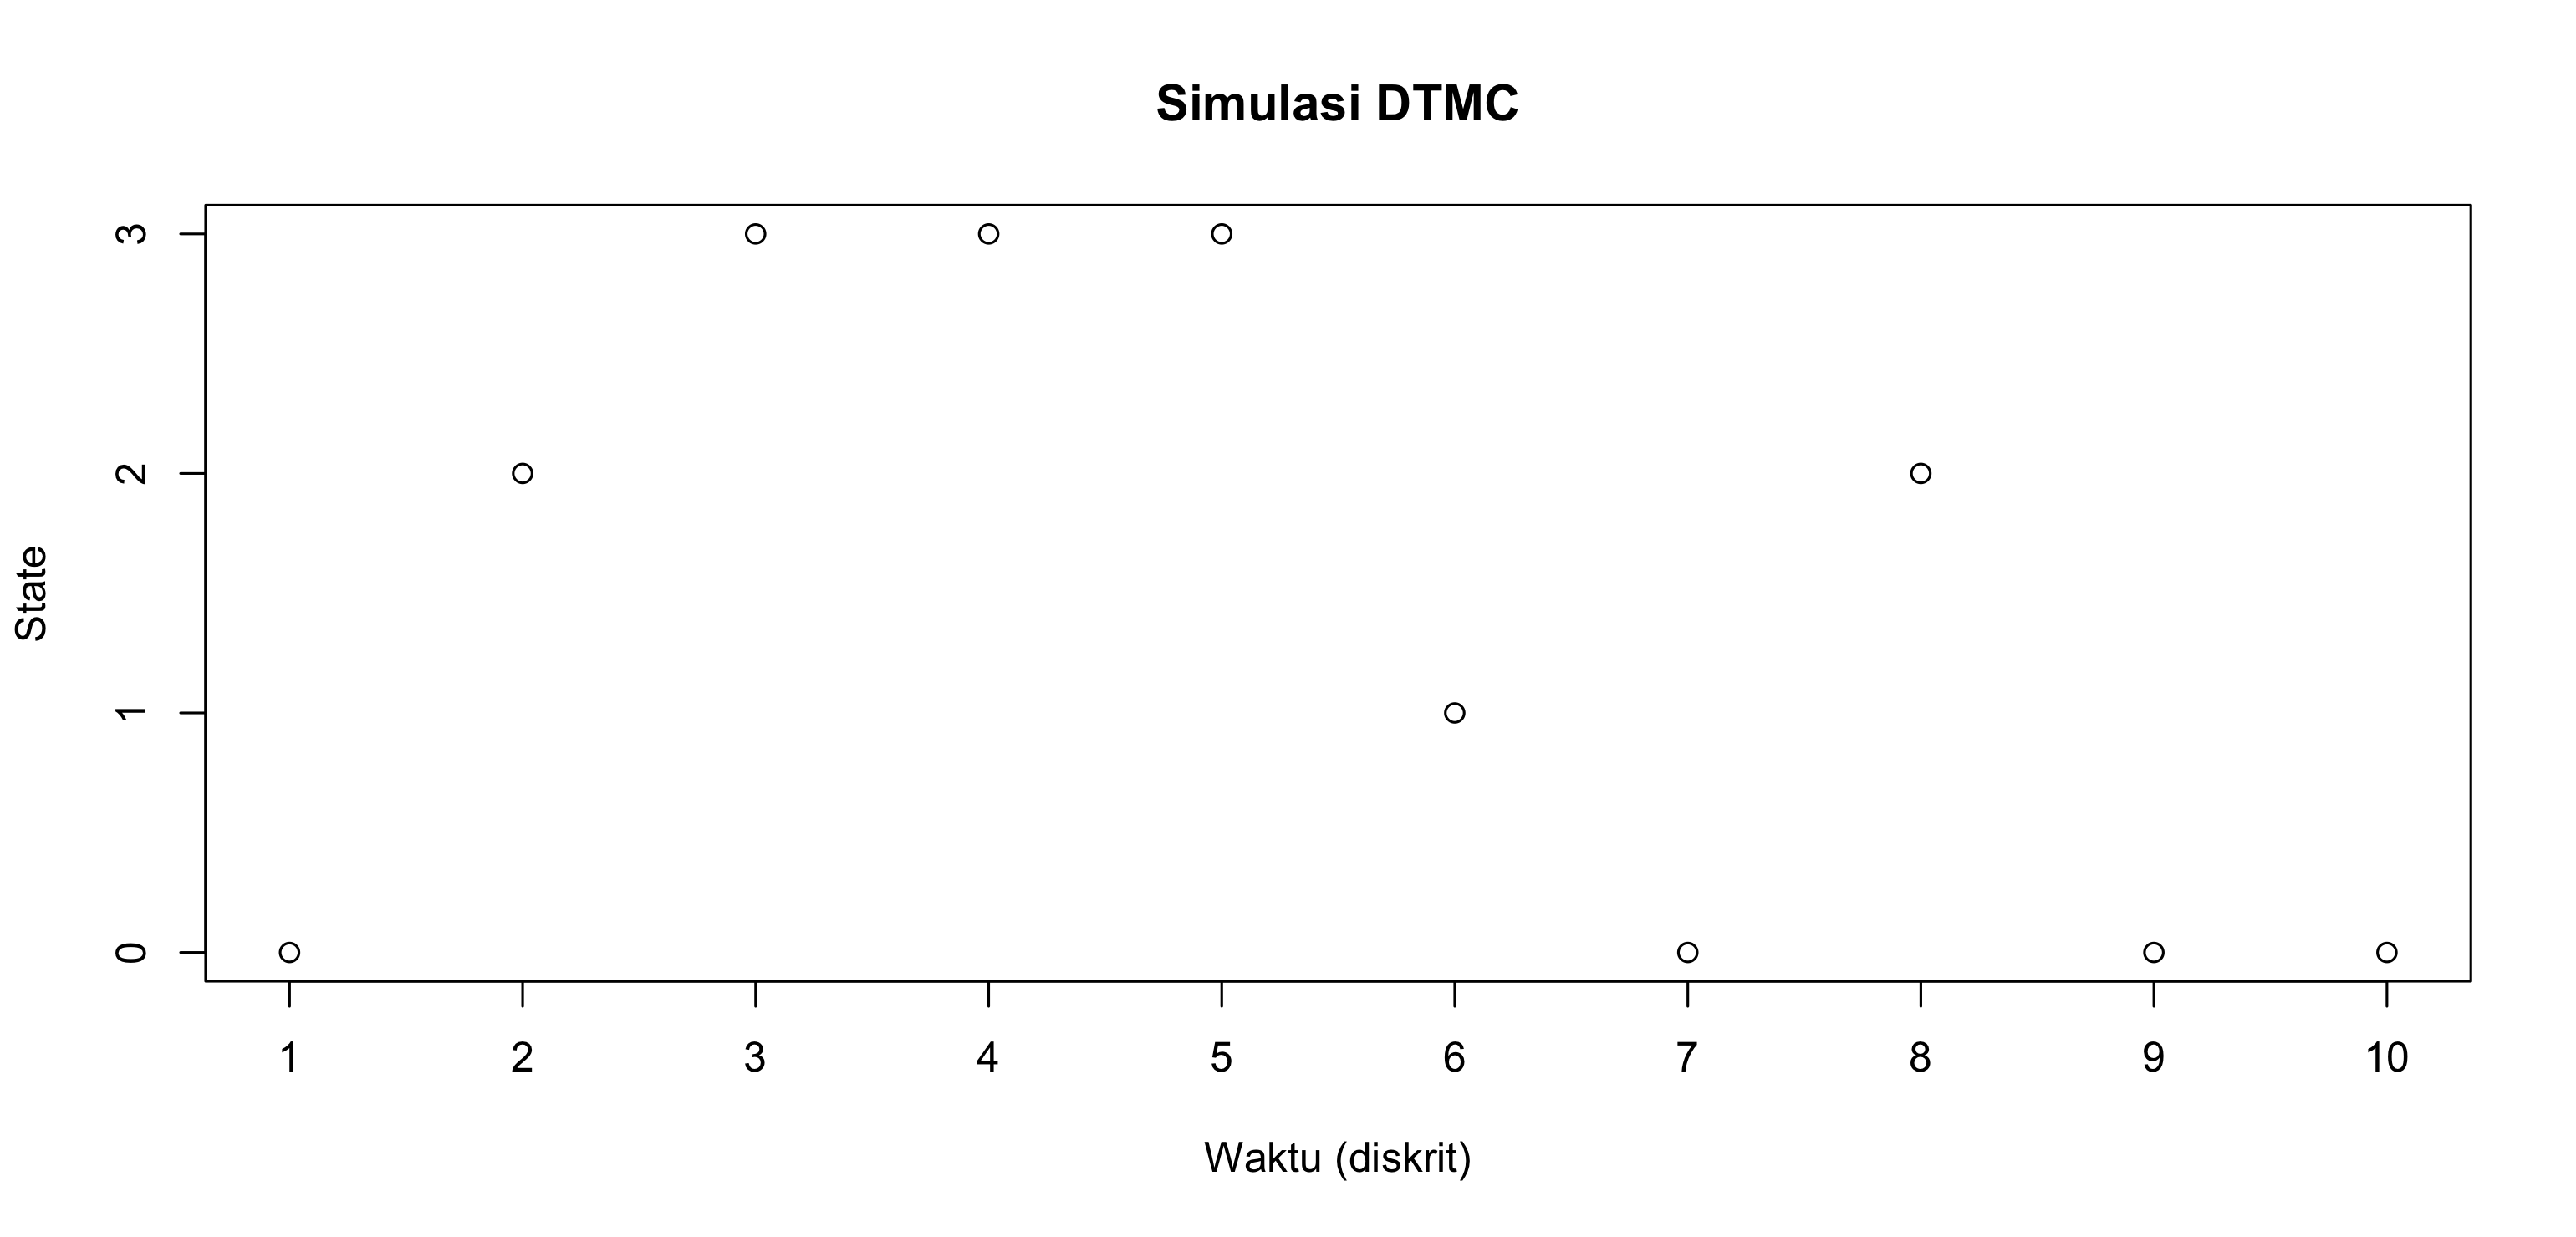
\includegraphics[scale=0.45]{gambar/contoh_dtmc_simulasi.png}
\end{frame}

\begin{frame}[fragile]{Probabilitas Jangka Panjang DTMC di R}
    Walaupun berupa proses \textit{random}, model stokastik memiliki konsep "probabilitas jangka panjang" \textit{(long-run probability)}, yaitu hitungan probabilitas secara umum berada di \textit{state} tertentu. Untuk itu, distribusi stasioner \textit{(stationary distribution)}, juga disebut \textit{steady state probabilities}, bisa dihitung.

    Di R, untuk DTMC, kita bisa memperoleh \textit{steady state probabilities} dengan

\begin{minted}{r}
steadyStates(mc1_obj)
\end{minted}

    Untuk contoh DTMC yang dibahas, hasilnya adalah

\begin{verbatim}
0         1         2         3
0.2352941 0.2352941 0.2352941 0.2941176
\end{verbatim}
    yang bisa ditulis \(p_n\) untuk \textit{steady state probability} untuk \textit{state} \(n\).
    \begin{align*}
        p_0 &\approx 0.2352941, & p_2 &\approx 0.2352941, \\
        p_1 &\approx 0.2352941, & p_3 &\approx 0.2941176
    \end{align*}
    \textbf{Catatan:} hasil bisa tergantung \textit{state} awal.
\end{frame}

\begin{frame}[fragile]{Analisis DTMC di R}
    Selain \textit{steady state probabilities}, beberapa hasil lainnya tentang DTMC juga bisa diperoleh di R, dengan fungsi \verb|summary|

\begin{minted}{r}
summary(mc1_obj)    
\end{minted}

    Hasilnya mengandung beberapa unsur DTMC yang tidak akan kita bahas di sini:

\begin{verbatim}
Unnamed Markov chain  Markov chain that is composed by: 
Closed classes: 
0 1 2 3 
Recurrent classes: 
{0,1,2,3}
Transient classes: 
NONE 
The Markov chain is irreducible 
The absorbing states are: NONE
\end{verbatim}
\end{frame}

\begin{frame}{Iklan: Kuliah Model Stokastik 1}
Di sini, kita membahas DTMC hanya sebagai pengantar untuk konsep-konsep model stokastik lainnya yang pada akhirnya berujung ke teori antrian, seperti diagram transisi. Apabila tertarik untuk mempelajari lebih lanjut, seperti tentang
\begin{itemize}
    \item pemodelan untuk berbagai persoalan menggunakan DTMC hingga penyelesaiannya,
    \item jenis-jenis \textit{state} seperti \textit{recurrent state}, \textit{transient state}, dan \textit{absorbing state}, serta
    \item sifat-sifat rantai Markov, seperti \textit{irreducible} dan periodik,
\end{itemize}
itu semua dipelajari di kuliah Model Stokastik 1 (3 SKS) yang bisa diambil semester depan (\textit{request} saja), saat ini merupakan mata kuliah wajib di semester genap (tepatnya semester 4) untuk program studi S1 Statistika dan program studi S1 Ilmu Aktuaria.

Sementara ini, kita akan lanjut membahas model stokastik yang lebih berkaitan dengan teori antrian, seperti proses Poisson.
\end{frame}

\subsection{Proses Poisson}

\begin{frame}{Distribusi Poisson}
    \begin{itemize}
        \item Proses Poisson didasari oleh distribusi Poisson, yang akan kita bahas terlebih dahulu
        \item Distribusi Poisson adalah distribusi diskrit yang memodelkan probabilitas untuk banyaknya kemunculan dalam suatu satuan waktu
        \item Hanya memliki satu parameter: rata-rata kemunculan per satuan waktu, biasa disebut \textit{rate} dan ditulis \( \lambda \), dengan syarat \( \lambda > 0 \)
        \item Contoh: \( \text{Pois}(3) \), yaitu distribusi Poisson dengan \textit{rate} \( \lambda = 3 \)

        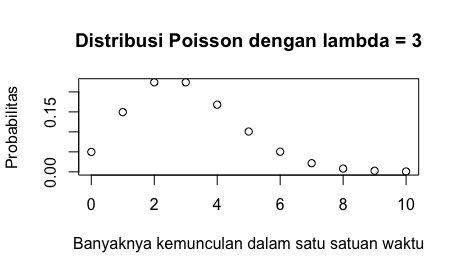
\includegraphics[scale=0.45]{gambar/dist_pois_lambda3.png}
    \end{itemize}
\end{frame}

\begin{frame}{PMF untuk Distribusi Poisson}
    %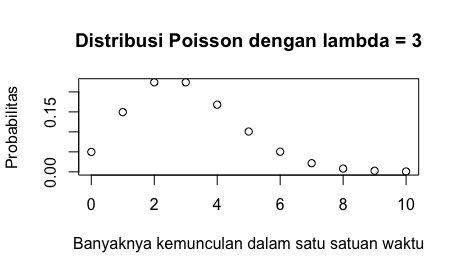
\includegraphics[scale=0.4]{gambar/dist_pois_lambda3.png}

    Misalkan variabel acak \(X\) berdistribusi Poisson dengan \textit{rate} \(\lambda\), atau biasa ditulis
    \[ X \sim \text{Pois}(\lambda) \]
    Gambar di atas adalah contoh gambar PMF \textit{(probability mass function)} dari distribusi Poisson, yaitu nilai probabilitas untuk tepat \(k\) kemunculan dalam satu satuan waktu:
    \[ \text{Pr}(X=k) = \frac{e^{-\lambda} \lambda^k}{k!} \]
    Contohnya, nilai PMF di \(k=2\) untuk \(\lambda = 3\) orang/menit adalah
    \[ \text{Pr}(X=2) = \frac{e^{-3} 3^2}{2!} \approx 0.2240418 \]
    yaitu probabilitas datangnya \textbf{tepat dua} orang dalam satu menit, jika rata-rata kedatangan adalah \(\lambda = 3\) orang/menit.
\end{frame}

\begin{frame}{CDF untuk Distribusi Poisson}
    Sebagaimana distribusi diskrit pada umumnya, CDF \textit{(cumulative distribution function)} untuk distribusi Poisson adalah sumasi PMF hingga nilai \(k\) yang ditentukan, ditulis \(\text{Pr}(X \le k)\)
    \[ \text{Pr}(X \le k) = \sum_{j=0}^{k} \text{Pr}(X = j) = \sum_{j=0}^{k} \frac{e^{-\lambda} \lambda^j}{j!} = \frac{e^{-\lambda} \lambda^0}{0!} + \dots + \frac{e^{-\lambda} \lambda^k}{k!} \]
    Interpretasinya di sini adalah probabilitas kemunculan \textbf{paling banyak} \(k\) dalam suatu satuan waktu.

    Contohnya, nilai CDF di \(k = 2\) untuk \( \lambda = 3 \) orang/menit adalah
    \begin{align*}
        \text{Pr}(X \le 2) &= \sum_{j=0}^{2} \frac{e^{-3} 3^j}{j!} = \frac{e^{-3} 3^0}{0!} + \frac{e^{-3} 3^1}{1!} + \frac{e^{-3} 3^2}{2!} \\
        &\approx 0.04978707 + 0.1493612 + 0.2240418 \\
        &\approx 0.4231901
    \end{align*}
    yaitu probabilitas datangnya \textbf{paling banyak dua} orang dalam satu menit, jika rata-rata kedatangan adalah \(\lambda = 3\) orang/menit.
\end{frame}

\begin{frame}[fragile]{PDF dan CDF Poisson di R}
    Untuk distribusi Poisson, R menyediakan fungsi \verb|dpois| untuk PMF dan \verb|ppois| untuk CDF. Misalnya, kita bisa menghitung \( \text{Pr}(X=2) \) dengan
\begin{minted}{r}
dpois(2, lambda = 3)
\end{minted}
    Hasil: \verb|0.2240418|

    Kita bisa menghitung \( \text{Pr}(X \le 2) \) dengan
\begin{minted}{r}
ppois(2, lambda = 3)
\end{minted}
    Hasil: \verb|0.4231901|

    atau bisa juga secara "manual" sebagai sumasi PMF, dan diperoleh hasil yang sama:
\begin{minted}{r}
dpois(0, lambda = 3) +
  dpois(1, lambda = 3) +
  dpois(2, lambda = 3)
\end{minted}
\end{frame}

\begin{frame}[fragile]{Plot Distribusi Poisson di R}
    Plot PMF \(\text{Pois}(3)\) di beberapa \textit{slide} sebelumnya diperoleh dengan kode R berikut. Intinya, kita memang menghitung nilai PMF Poisson di \(0, \dots, 10\), kemudian menampilkannya.

\begin{minted}[fontsize=\small]{r}
par_lambda <- 3
x_pois <- 0 : 10
p_pois <- dpois(x_pois, lambda = par_lambda)
plot(x_pois, p_pois,
     main = "Distribusi Poisson dengan lambda = 3",
     xlab = "Banyaknya kemunculan dalam satu satuan waktu",
     ylab = "Probabilitas")
\end{minted}

    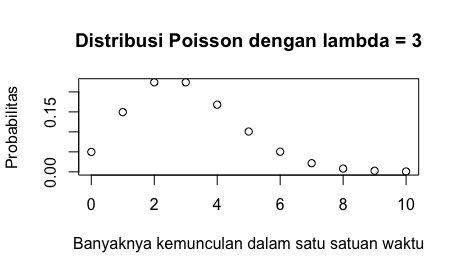
\includegraphics[scale=0.4]{gambar/dist_pois_lambda3.png}
\end{frame}

\begin{frame}{Sifat-Sifat Distribusi Poisson}
    Untuk variabel acak \(X \sim \text{Pois}(\mu)\), berlaku
    \begin{itemize}
        \item \(\text{E}\brackets{X} = \mu\), yaitu ekspektasi atau rata-rata untuk \(X\) adalah \(\mu\)
        \item \(\text{Var}\brackets{X} = \mu\), yaitu variansi untuk \(X\) juga \(\mu\)
    \end{itemize}
    sehingga \(\text{E}\brackets{X} = \text{Var}\brackets{X} = \mu\).

    Oleh karena itu, distribusi Poisson \(\text{Pois}(\lambda)\) terkadang disebut "memiliki parameter \(\lambda\)", "memiliki \textit{rate} \(\lambda\)", atau "memiliki rata-rata \(\lambda\)", artinya sama.

    Selain itu, hasil jumlah dua variabel acak independen yang berdistribusi Poisson juga berdistribusi Poisson dengan \textit{rate} berupa hasil jumlah dari kedua \textit{rate}, atau bisa ditulis
    \[\text{Pois}(\mu) + \text{Pois}(v) \sim \text{Pois}(\mu + v)\]
    %selama \(\text{Pois}(\mu)\) dan \(\text{Pois}(v)\) independen, karena

    Penggunaan distribusi Poisson untuk memodelkan kemunculan dirumuskan sebagai model stokastik bernama proses Poisson, dibahas setelah ini.
\end{frame}

\begin{frame}{Definisi Proses Poisson}
    Proses Poisson dengan \textit{rate} \(\lambda > 0\) adalah model stokastik bernilai bulat, misalnya dinotasikan \( \braces{X(t); \, t \ge 0} \) dengan \(X(t)\) melambangkan banyaknya kemunculan dari waktu nol sampai \(t\), yang memenuhi
    \begin{itemize}
        \item \(X(0) = 0\), yaitu belum ada kemunculan di waktu \(t=0\);
        \item \textit{independent increments}, yaitu variabel-variabel acak berikut (masing-masing berupa selisih kemunculan, yaitu banyaknya kemunculan dalam interval waktu)
        \[ X\pars{t_i} - X\pars{t_{i-1}}, \quad 0 \le t_1 < t_2 < \dots < t_n \]
        semuanya saling independen; dan
        \item untuk tiap titik waktu \(s \ge 0\) dan durasi \(t > 0\), berlaku
        \[X(s+t) - X(s) \sim \text{Pois}(\lambda t)\]
        yaitu banyaknya kemunculan dalam interval waktu \(\brackets{s,s+t}\) berdistribusi \(\text{Pois}(\lambda t)\)
    \end{itemize}
\end{frame}

\begin{frame}{Sifat-Sifat Proses Poisson}
    Jelas bahwa \(\text{E}\brackets{X(t)} = \text{Var}\brackets{X(t)} = \lambda t\) karena
    \[X(t) = X(0+t) - X(0) \sim \text{Pois}(\lambda t)\]
    Selain itu, untuk tiap titik waktu \(s \ge 0\) dan durasi \(t > 0\), berlaku
    \[\text{Pr}\brackets{X(s+t) - X(s) = k} = \frac{e^{-\lambda t}\pars{\lambda t}^k}{k!}\]
    sesuai rumus PMF Poisson, tepatnya \(\text{Pois}(\lambda t)\). Maka,
    \[\text{Pr}\brackets{X(t) = k} = \text{Pr}\brackets{X(0+t) - X(0) = k} = \frac{e^{-\lambda t}\pars{\lambda t}^k}{k!}\]
    sehingga bisa disimpulkan
    \[\text{Pr}\brackets{X(s+t) - X(s) = k} = \text{Pr}\brackets{X(t) = k} = \frac{e^{-\lambda t}\pars{\lambda t}^k}{k!}\]
\end{frame}

\begin{frame}{\textit{Stationary increments} dalam proses Poisson}
    Untuk proses Poisson \(\braces{X(t)}\), sudah ditunjukkan bahwa
    \[\text{Pr}\brackets{X(s+t) - X(s) = k} = \text{Pr}\brackets{X(t) = k}\]
    Pilih \(b = s+t\) dan \(a = s\) agar \(t = b-s = b-a\), sehingga
    \[\text{Pr}\brackets{X(b) - X(a) = k} = \text{Pr}\brackets{X\pars{b-a} = k}\]
    Kedua persamaan di atas adalah sifat yang sama, yang disebut \textit{stationary increments}.
    %\textbf{Kesamaan probabilitas mengindikasikan kesamaan PMF, yang mengimplikasikan kesamaan distribusi.}
\end{frame}

\begin{frame}{\textit{Interarrival times} dan \textit{waiting/arrival times}}
    Sejauh ini, kita berurusan dengan banyaknya kemunculan dalam interval waktu.
    
    Kita juga bisa membalikkannya, agar berurusan dengan lama waktu antar kemunculan, juga disebut waktu antar kedatangan \textit{(interarrival time)} atau \textit{sojourn time}, biasa dilambangkan \( T_n \) untuk durasi antara kemunculan ke-\((n-1)\) dengan kemunculan ke-\(n\). Karena kemunculan di sini bersifat acak, \textit{interarrival time} \(T_n\) juga berupa variabel acak, dan \(\braces{T_n, \, n=1,2,\dots}\) menjadi barisan variabel acak, disebut barisan \textit{interarrival times}, dimulai dari \(T_1\) sebagai durasi dari awal dimulainya proses Poisson hingga kemunculan pertama. Tiap \(T_i\) saling independen.

    Terkadang, kita ingin berurusan dengan lama waktu dari awal proses hingga kedatangan ke-\(n\), daripada lama waktu antar kedatangan. Untuk itu, variabel acak \textit{waiting time} atau \textit{arrival time} didefinisikan
    \[W_n = T_1 + T_2 + \dots + T_n\]
\end{frame}

\begin{frame}{\(T_1\) berdistribusi eksponensial}
    Bagaimana distribusi dari \(T_n\)? Mari kita tinjau \(T_1\) terlebih dahulu. Kita bisa tinjau CDFnya yaitu \(\text{Pr}(T_1 \le t)\), lalu kita hubungkan dengan kemunculan: kejadian \(\brackets{T_1 \le t} = \brackets{W_1 \le t}\), bahwa kemunculan pertama sudah tercapai, itu sama saja dengan kejadian \(\brackets{X(t) \ne 0}\), yaitu banyaknya kemunculan sudah tidak lagi nol. Maka probabilitas kedua kejadian sama, sehingga
    \begin{align*}
        \text{Pr}\pars{T_1 \le t} &= \text{Pr}\brackets{X(t) \ne 0}
        = 1 - \text{Pr}\brackets{X(t) = 0}
        = 1 - \frac{e^{-\lambda t}\pars{\lambda t}^0}{0!} \\
        &= 1 - \frac{e^{-\lambda t}(1)}{1}
        = 1 - e^{-\lambda t}
    \end{align*}
    yaitu CDF distribusi eksponensial (mari kita bahas!), sehingga \(T_1 \sim \text{Exp}(\lambda)\), yaitu variabel acak \(T_1\) berdistribusi eksponensial dengan parameter \(\lambda\) yang juga disebut \textit{rate}.
\end{frame}

\begin{frame}{Distribusi Eksponensial}
    Distribusi eksponensial adalah suatu distribusi kontinu dengan satu parameter saja, biasa ditulis \(\lambda > 0\) (kebetulan?), dan biasa disebut \textit{rate} (kebetulan?). Apabila dimisalkan
    \[T \sim \text{Exp}(\lambda)\]
    yaitu \(T\) berdistribusi eksponensial dengan \textit{rate} \(\lambda\), bisa ditulis fungsi PDF \textit{(probability density function)}
    \[f_T(t) = \begin{cases}
        \lambda e^{-\lambda t}, & t \ge 0 \\
        0, & t < 0
    \end{cases}\]
    dan CDF berikut (dihitung sebagai integral dari \(-\infty\) sampai \(t\) dari PDF, sebagaimana distribusi kontinu pada umumnya)
    \[F_T(t) = \text{Pr}(T \le t) = \begin{cases}
        1 - e^{-\lambda t}, & t \ge 0 \\
        0, & t < 0
    \end{cases}\]
\end{frame}

\begin{frame}{Sifat-Sifat Distribusi Eksponensial}
    Untuk variabel acak \(T \sim \text{Exp}(\lambda)\), berlaku
    \[\text{E}\brackets{T} = \frac{1}{\lambda}, \quad \text{Var}\brackets{T} = \frac{1}{\lambda^2}\]
    sehingga \(\text{Var}\brackets{T} = \text{E}\brackets{T}^2\).

    Daripada menulis CDF eksponensial yaitu \(\text{Pr}(T \le t) = 1 - e^{-\lambda t}\), lazim ditulis
    \[\text{Pr}(T > t) = e^{-\lambda t}\]

    %Selain itu, apabila variabel-variabel acak \(T_1, \dots, T_n\) saling independen dan \(T_i \sim \text{Exp}(\lambda_i)\) untuk \(i=1,\dots,n\), maka \[\text{min}\braces{T_1, \dots, T_n} \sim \text{Exp}\pars{\lambda_1 + \dots + \lambda_n}\]
    Yang terpenting, distribusi eksponensial adalah \textbf{satu-satunya distribusi kontinu yang memenuhi \textit{memoryless property}} sebagai berikut:
    \[\text{Pr}\pars{T > t+s \; \middle| \; T > s} = \text{Pr}\pars{T > t}\]
    untuk titik waktu \(s \ge 0\) dan durasi \(t > 0\), karena
    \begin{align*}
        \text{Pr}\pars{T > t+s \; \middle| \; T > s} &= \frac{\text{Pr}\pars{T>t+s, T>s}}{\text{Pr}\pars{T>s}} = \frac{\text{Pr}\pars{T>t+s}}{\text{Pr}\pars{T>s}} \\
        &= \frac{e^{-\lambda \pars{t+s}}}{e^{-\lambda s}} = e^{-\lambda t} = \text{Pr}\pars{T > t}
    \end{align*}
\end{frame}

% (cara salah, batal)
%\begin{frame}{\(T_n\) berdistribusi eksponensial}
    %Dengan cara yang serupa seperti \(T_1\), mari kita tinjau distribusi \(T_n\). Kejadian \(\brackets{T_n \le t}\), bahwa kemunculan ke-\(n\) sudah tercapai, sama dengan kejadian \(\brackets{X(t) \ge n}\), yaitu banyaknya kemunculan hingga titik waktu \(t\) setidaknya sebanyak \(n\), sehingga
    %\begin{align*}
        %\text{Pr}\pars{T_n \le t} &= \text{Pr}\brackets{X(t) \ge n} = 1 - \text{Pr}\brackets{X(t) < n} \\
        %&= 1 - \sum_{j=0}^{n-1} \text{Pr}\brackets{X(t) = j} = 1 - \sum_{j=0}^{n-1} \frac{e^{-\lambda t}\pars{\lambda t}^j}{j!}
    %\end{align*}
    %Mengingat bahwa jumlahan distribusi Poisson yang saling independen juga berdistribusi Poisson dengan \textit{rate} yang dijumlah,
    %\[\text{Pr}\pars{T_n \le t} = 1 - \sum_{j=0}^{n-1} \frac{e^{-\lambda t}\pars{\lambda t}^j}{j!} = 1 - \frac{e^{-n\lambda t}\pars{n\lambda t}^j}{j!}\]
%\end{frame}
% (salah juga)
%\begin{frame}{\(T_n\) berdistribusi eksponensial}
    %Sekarang, mari kita tinjau distribusi \(T_n\). Perhatikan bahwa \(T_n = W_n - W_{n-1}\), sehingga berdasarkan \textit{memoryless property} dari distribusi \(T \sim \text{Exp}(\lambda)\),
    %\begin{align*}
        %\text{Pr}\brackets{T > W_{n-1} + T_n \; \middle| \; T > T_n} = \text{Pr}\pars{T > W_{n-1}}
    %\end{align*}
%\end{frame}
% (gagal lagi, au ah)
%\begin{frame}{\(T_n\) berdistribusi eksponensial}
    %Dengan cara yang mirip seperti \(T_1\), mari kita tinjau distribusi \(T_n\). Namun, daripada meninjau CDF yaitu \(\text{Pr}\pars{T_n \le t}\), kita tinjau \(\text{Pr}\pars{T_n > t}\).
    %Kejadian \(\brackets{T_n > t}\), bahwa kemunculan ke-\(n\) belum tercapai, sama dengan kejadian \(\brackets{X(t) < n}\), yaitu banyaknya kemunculan hingga titik waktu \(t\) masih kurang dari \(n\). Sehingga, %Perhatikan bahwa \(T_n = W_n - W_{n-1}\).
    %\begin{align*}
        %\text{Pr}\pars{T_n \le t} &= \text{Pr}\brackets{X(t) < n} = \text{Pr}\brackets{X\pars{t - W_{n-1} + W_{n-1}} < n}
    %\end{align*}
    %Berdasarkan sifat proses Poisson,
    %\begin{align*}
        %\text{Pr}\brackets{X\pars{t - W_{n-1} + W_{n-1}} - X\pars{W_{n-1}} < n} = \text{Pr}\brackets{X\pars{t - W_{n-1}} < n}
    %\end{align*}
%\end{frame}
% menggeser meragukan...
%\begin{frame}{\(T_n\) berdistribusi eksponensial}
    %Dengan cara yang mirip seperti \(T_1\), mari kita tinjau distribusi \(T_n\). Namun, daripada meninjau CDF yaitu \(\text{Pr}\pars{T_n \le t}\), kita tinjau \(\text{Pr}\pars{T_n > t}\). Kejadian \(\brackets{T_n > t}\), bahwa kemunculan ke-\(n\) belum tercapai, sama dengan kejadian \(\brackets{X(t) < n}\), yaitu banyaknya kemunculan hingga titik waktu \(t\) masih kurang dari \(n\). Sehingga,
    %\begin{align*}
        %\text{Pr}\pars{T_n > t} &= \text{Pr}\brackets{X(t) < n} = \text{Pr}\brackets{X(t) - (n-1) < n - (n-1)} \\
        %&= \text{Pr}\brackets{X(t) - X\pars{W_{n-1}} < 1} = \text{Pr}\brackets{X(t) - X\pars{W_{n-1}} = 0} \\
        %%&= \text{Pr}\brackets{X\pars{t - W_{n-1} + W_{n-1}} - X\pars{W_{n-1}} = 0} \\
        %&\text{Berdasarkan sifat \textit{stationary increments},} \\
        %&= \text{Pr}\brackets{X\pars{t - W_{n-1}} = 0} \\
        %&\text{"Menggeser" proses Poisson ke kemunculan ke-}(n-1), \\
        %&= \text{Pr}\brackets{X(t) = 0} = \frac{e^{-\lambda t}\pars{\lambda t}^0}{0!} = e^{-\lambda t}
    %\end{align*}
    %Dengan demikian, \(T_n \sim \text{Exp}(\lambda)\).
%\end{frame}
% ALL THIS TIME I BEGAN WITH T_n > t AND THOUGHT IT MEANT THE WAITING TIME IS MORE THAN t........ YET SOMEHOW I KNEW, FOR ALL STEPS AFTER THAT, THAT T_n IS INTERARRIVAL... NO WONDER I KEEP GETTING IT WRONG THE WHOLE DAY DAMN IT!
%\begin{frame}{\(T_n\) berdistribusi eksponensial}
    %Dengan cara yang mirip seperti \(T_1\), mari kita tinjau distribusi \(T_n\) melalui CDF.
    %%Namun, daripada meninjau CDF yaitu \(\text{Pr}\pars{T_n \le t}\), kita tinjau \(\text{Pr}\pars{T_n > t}\). Kejadian \(\brackets{T_n > t}\), bahwa kemunculan ke-\(n\) belum tercapai, sama dengan kejadian \(\brackets{X(t) < n}\), yaitu banyaknya kemunculan hingga titik waktu \(t\) masih kurang dari \(n\).
    %Kejadian \(\brackets{T_n \le t}\), bahwa kemunculan ke-\(n\) sudah tercapai, sama dengan kejadian \(\brackets{X(t) \ge n}\), yaitu banyaknya kemunculan hingga titik waktu \(t\) setidaknya sudah sebanyak \(n\).
    %%Lebih tepatnya, untuk mempermudah, kita misalkan \(T_{n-1} = s\) sehingga \(0 < s < t\), yaitu 
    %Dengan demikian, \(T_n \sim \text{Exp}(\lambda)\).
%\end{frame}
% let's get it right this time
\begin{frame}{\(T_n\) berdistribusi eksponensial}
    Mari kita tinjau distribusi \(T_n\). Karena distribusi \(T_1\) sudah diketahui, kita bisa mencoba pendekatan perbandingan. Kita juga bisa meninjau probabilitas \(\brackets{T_2 > t}\) daripada CDF \(\brackets{T_2 \le t}\).
    
    Misalkan \(s > 0\) dan \(t > 0\) adalah dua durasi, misalnya untuk dua kemunculan berturut-turut. Perhatikan bahwa \( (0,s] \) dan \( (s, s+t] \) adalah dua interval yang saling lepas karena \( 0 < s < s+t \), sehingga berdasarkan sifat \textit{independent increments}, variabel acak \(X\pars{s+t} - X\pars{s}\) dan \(X\pars{s} - X\pars{0} = X\pars{s}\) saling bebas; 
    %Sehingga, apabila kita hitung probabilitas bersyarat seperti berikut, syarat akan hilang:
    apabila dihitung probabilitas bersyarat seperti berikut, syarat hilang:
    \begin{align*}
        \text{Pr}\pars{T_2 > t \; \middle| \; T_1 = s} &= \text{Pr}\brackets{X\pars{s+t} - X\pars{s} = 0 \; \middle| \; X\pars{s} = 1 } \\
        &= \text{Pr}\brackets{X\pars{s+t} - X\pars{s} = 0} \quad \pars{= \text{Pr}\pars{T_2 > t}} \\
        &\text{Berdasarkan sifat \textit{stationary increments,}} \\
        &= \text{Pr}\brackets{X\pars{t} = 0} = \frac{e^{-\lambda t} \pars{\lambda t}^0}{0!} = e^{-\lambda t}
    \end{align*}
    sehingga \(T_2 \sim \text{Exp}(\lambda)\). Dengan bukti serupa, \(T_n \sim \text{Exp}(\lambda)\).
    %Dengan bukti serupa, dapat disimpulkan \(T_n \sim \text{Exp}(\lambda)\) untuk \(n = 1, 2, 3, \dots\)
\end{frame}

\begin{frame}{Contoh Proses Poisson: Kedatangan Pelanggan}
    Kedatangan pelanggan di toko tertentu mengikuti proses Poisson dengan \textit{rate} \(\lambda = 4\) orang/jam. Toko buka pukul 09.00 pagi. Tentukan probabilitas bahwa tepat satu pelanggan telah datang ketika sudah pukul 09.30 pagi DAN tepat lima pelanggan telah datang ketika sudah pukul 11.30 siang.

    \textbf{Jawab:} misalkan \(t\) bersatuan jam (agar \(\lambda = 4\) orang/jam), dan dipasang \(t=0\) untuk pukul 09.00. Memanfaatkan \textit{independent increments} antar variabel acak \(X\pars{\frac{5}{2}} - X\pars{\frac{1}{2}}\) dengan \(X\pars{\frac{1}{2}}\),
    \begin{align*}
        \text{Pr}&\braces{X\pars{\frac{1}{2}} = 1, \, X\pars{\frac{5}{2}} = 5} \\
        &= \text{Pr}\braces{X\pars{\frac{1}{2}} = 1, \, X\pars{\frac{5}{2}} - X\pars{\frac{1}{2}} = 5-1} \\
        &= \text{Pr}\braces{X\pars{\frac{1}{2}} = 1} \text{Pr}\braces{X\pars{2} = 4} \\
        &= \braces{ \frac{e^{-4(1/2)} \pars{4(1/2)}^1}{1!} }\braces{ \frac{e^{-4(2)} \pars{4(2)}^4}{4!} }
        %= \pars{2e^{-2}} \pars{\frac{512}{3}e^{-8}}
        \approx 0.0154965
    \end{align*}
\end{frame}

\begin{frame}{Simulasi Proses Poisson}
    Simulasi proses Poisson bisa dilakukan dengan langkah-langkah berikut.
    \begin{enumerate}
        \item Tetapkan \textit{rate} \(\lambda\) dan banyaknya kemunculan \(n\) yang ingin disimulasikan, lalu hasilkan barisan \textit{interarrival times} \(\braces{T_i, \, i = 1, \dots, n}\) dengan menarik \(n\) buah data \textit{random} dari \(\text{Exp}(\lambda)\).
        \item Susun barisan \textit{arrival times} \(\braces{W_i, \, i = 1, \dots, n}\) dengan menghitung jumlahan kumulatif atau \textit{cumulative sum} sesuai definisi:
        \[W_i = T_1 + \dots + T_i\]
        \item Tampilkan \textit{plot} kemunculan ke-\(i\), \( i = 1, \dots, n \) terhadap barisan \textit{arrival times}, sebagai \textit{plot} hasil simulasi kemunculan agar bisa melihat kapan munculnya.
    \end{enumerate}
\end{frame}

\begin{frame}[fragile]{Simulasi Proses Poisson di R}
    Menetapkan \(\lambda\) dan \(n\),
\begin{minted}{r}
pp_lambda <- 4
pp_n <- 10
\end{minted}
    Menghasilkan barisan \textit{interarrival times},
\begin{minted}{r}
set.seed(2024)
pp_interarrival <- rexp(pp_n, rate = pp_lambda)
\end{minted}
    Menyusun barisan \textit{arrival times},
\begin{minted}{r}
pp_arrival <- cumsum(pp_interarrival)    
\end{minted}
    Dengan \textit{seed} 2024, data hasil simulasi yang tersimpan di \verb|pp_arrival| adalah:
\begin{verbatim}
0.1684713 0.4126256 0.5028073 0.6018938 0.8472178
1.0737138 1.0943433 1.1837221 1.3761243 1.3988369
\end{verbatim}
\end{frame}

\begin{frame}[fragile]{Plot Hasil Simulasi Proses Poisson di R}
    Dengan sedikit kode, hasil simulasi proses Poisson bisa ditampilkan sebagai \textit{plot} kemunculan ke-\(i\) terhadap barisan \textit{arrival times}. Hasil \textit{plot} ditampilkan di \textit{slide} selanjutnya. (Kemunculan ke-"nol" dengan \textit{arrival time} "nol" juga "diadakan" hanya agar titik awal proses Poisson tergambarkan.)
\begin{minted}{r}
plot(x = c(0, pp_arrival),
     y = 0 : length(pp_arrival),
     type = "s",
     xlab = "Waktu",
     ylab = "Kedatangan",
     main = "Simulasi Proses Poisson dengan lambda = 4")
\end{minted}
\end{frame}

\begin{frame}{Plot Hasil Simulasi Proses Poisson di R}
    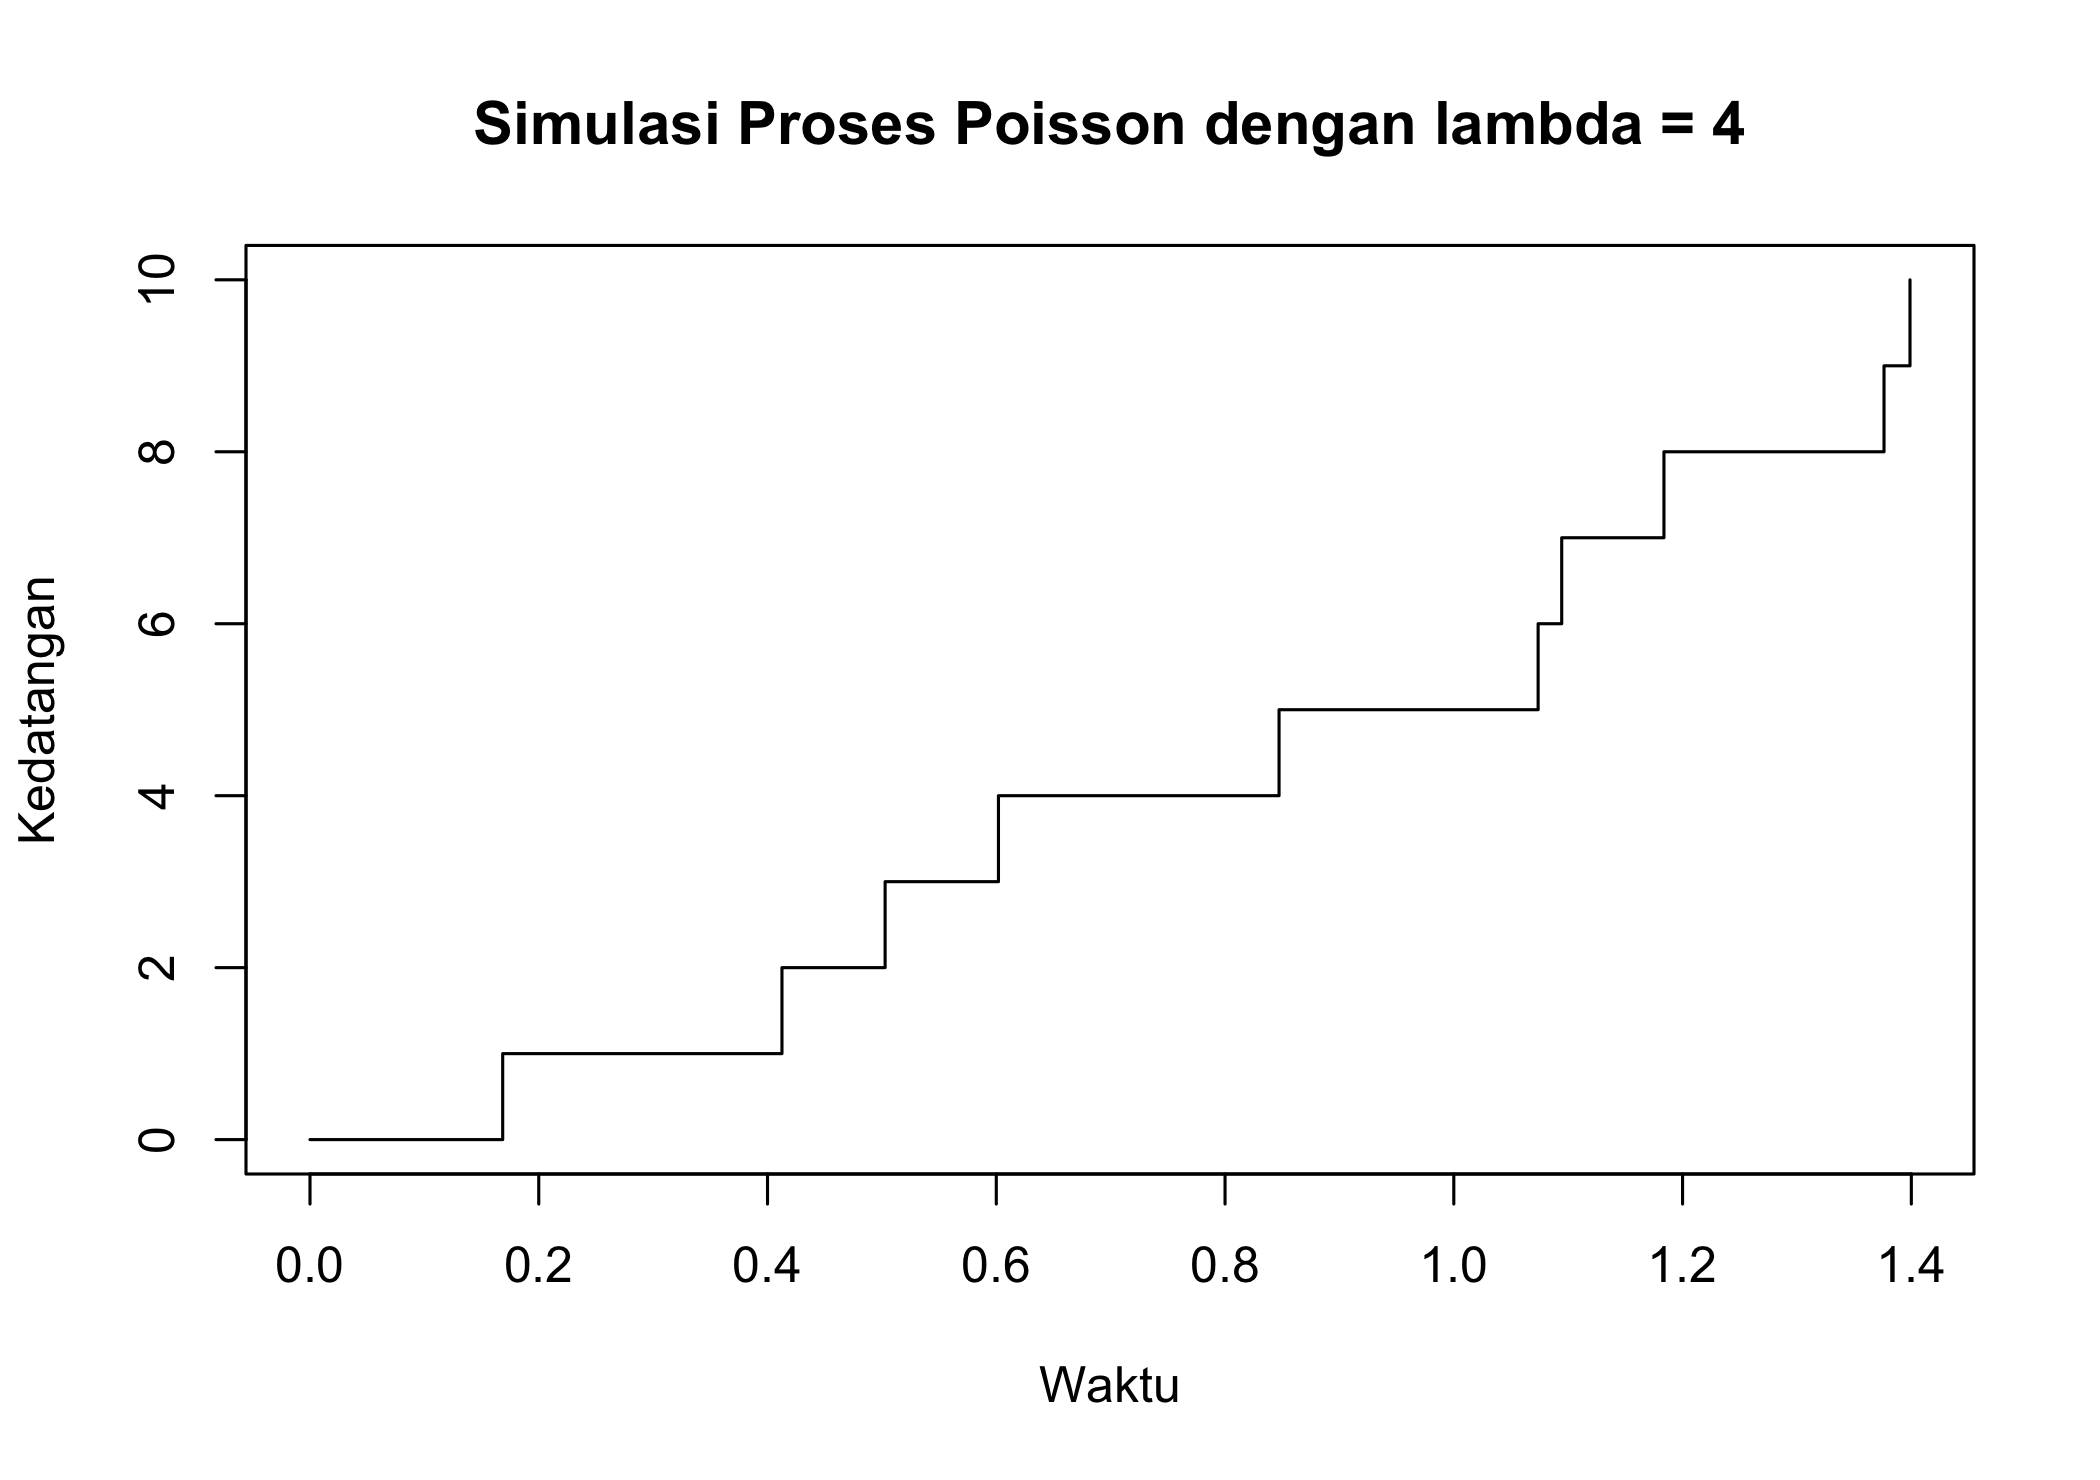
\includegraphics[scale=0.65]{gambar/proc_pois_lambda4_sim.png}
\end{frame}

\begin{frame}{Iklan (2): Kuliah Model Stokastik 1}
    Proses Poisson adalah model stokastik, sehingga juga dipelajari di kuliah Model Stokastik 1 (3 SKS) di samping DTMC. Selain dasar teori yang lebih mendalam, seperti mempelajari konsep \textit{counting process} yang mendasarinya atau bahkan notasi \textit{little-o}, berbagai contoh pemodelan dan aplikasi proses Poisson juga dibahas di sana, sedangkan di sini hanya dibahas sebagian tentang proses Poisson untuk menunjang perkuliahan tentang teori antrian. Apabila tertarik mempelajari lebih lanjut, silakan ambil kuliah Model Stokastik 1 semester depan. \\[0.5em]
    
    Bagaimanapun juga, proses Poisson sebenarnya adalah kasus khusus dari CTMC, yang selanjutnya kita bahas.
\end{frame}

\subsection{Rantai Markov Waktu Kontinu (CTMC)}

\begin{frame}{Definisi CTMC}
    \begin{itemize}
        \item CTMC melibatkan perpindahan \textit{state} sebagaimana DTMC, tapi memiliki hitungan waktu yang kontinu sebagaimana proses Poisson.
        \item CTMC bisa didefinisikan sebagai \textit{family of random variables} \(\braces{X(t); \, 0 \le t < \infty}\), dengan \textit{support} (nilai-nilai yang mungkin) berupa \textit{state space} terhitung misalnya \(S\), yang memenuhi \textbf{\textit{memoryless property}} berikut untuk tiap \(i, j \in S\), tiap titik waktu \(s \ge 0\), tiap durasi \(t \ge 0\), dan sembarang "riwayat" \(x(u)\) selama masa lalu \(0 \le u < s\),
        \begin{align*}
            \text{Pr}&\brackets{X\pars{t+s} = j \; \middle| \; X\pars{s} = i, \, X(u) = x(u), \, 0 \le u < s} \\
            &= \text{Pr}\brackets{X\pars{t+s} = j \; \middle| \; X\pars{s} = i}
        \end{align*}
        Intinya, masa depan \(t+s\) hanya dipengaruhi oleh masa kini \(s\), tidak oleh masa lalu \(0 \le u < s\).
        \item CTMC bisa transisi kapanpun, dengan \textit{transition probability function}
        \[P_{ij}\pars{t} = \text{Pr}\brackets{X\pars{t+s} = j \; \middle| \; X\pars{s} = i}\]
    \end{itemize}
\end{frame}

\begin{frame}{CTMC homogen}
    tes
\end{frame}

\subsection{\textit{Birth-Death Process}}

\subsection{Antrian dan Notasinya}

\section{Antrian M/M/c}

\subsection{M/M/c secara umum}

\subsection{Kasus khusus: Antrian M/M/1}

\subsection{Simulasi M/M/c di R}

\subsection{M/M/c di QtsPlus}

\section{Lampiran: Tautan, \textit{GitHub repository}, Referensi}

\begin{frame}{Tautan dan \textit{GitHub repository}}
    Untuk \textit{package} R yang digunakan:
    \begin{itemize}
        \item markovchain: \url{https://github.com/spedygiorgio/markovchain}

        \item queuecomputer: \url{https://github.com/AnthonyEbert/queuecomputer}
        
        \item queueing: \url{https://cran.r-project.org/web/packages/queueing/index.html}
    \end{itemize}

    Tautan lainnya:

    \begin{itemize}
        \item QtsPlus v4.0: \url{https://mason.gmu.edu/~jshortle/fqt5th.html}
        
        \item \textit{GitHub repository} untuk presentasi ini (termasuk kode): \url{https://github.com/BismaBRJ/intro_stokastik_antrian_r_2024/}
    \end{itemize}
\end{frame}

\begin{frame}{Referensi}
    \begin{itemize}
        \item Pinsky, Mark A. \& Karlin, Samuel (2011). \textit{An Introduction to Stochastic Modeling} (edisi ke-2). Elsevier.
        
        \textbf{Untuk:} sebagian besar materi DTMC, proses Poisson, dan CTMC, kecuali contoh dan simulasi dengan R

        \item Shortle, John F.; Thompson, James M.; Gross, Donald; \& Harris, Carl M. (2018). \textit{Fundamentals of Queueing Theory} (edisi ke-5). Wiley. \url{https://mason.gmu.edu/~jshortle/fqt5th.html}
        
        \textbf{Untuk:} sebagian besar materi \textit{birth-death process} dan antrian, termasuk M/M/c, kecuali contoh dan simulasi dengan R

        \textbf{Catatan:} sering disebut buku \textbf{Gross \& Harris} karena merekalah yang menulis edisi pertama
    \end{itemize}
\end{frame}

\end{document}